\documentclass{article}
\usepackage{amsmath}
\usepackage{xcolor}
\usepackage{ragged2e}
\usepackage{graphicx}
\usepackage{gensymb}
\usepackage{mathtools}
\newcommand{\mydet}[1]{\ensuremath{\begin{vmatrix}#1\end{vmatrix}}}
\providecommand{\brak}[1]{\ensuremath{\left(#1\right)}}
\providecommand{\norm}[1]{\left\lVert#1\right\rVert}
\newcommand{\solution}{\noindent \textbf{Solution: }}
\newcommand{\myvec}[1]{\ensuremath{\begin{pmatrix}#1\end{pmatrix}}}
\let\vec\mathbf
\begin{document}
\begin{center}
	\textbf\large{CHAPTER-7 \\ TRIANGLES}
\end{center}
\section{Exercise 7.1}
Q1. In quadrilateral $ACBD$, \begin{equation} AC = AD \end{equation} and $AB$ bisect $\angle{A}$ (see Fig.\ref{fig:Fig}). Show that $\triangle{ABC} \cong \triangle{ABD}$. What can you say about $BC$ and $BD$? 
\solution
It is given that $AC$ and $AD$ are equal i.e., \begin{equation} AC = AD \end{equation} and the line segment $AB$ bisects $\angle{A}$.\\
We will have to now prove that the two triangles $ABC$ and $ABD$ are similar i.e., \textbf{$\triangle{ABC} \cong \triangle{ABD}$}.\\
\textbf{Proof:}
Consider the triangles $\triangle{ABC}$ and $\triangle{ABD}$
\begin{enumerate}
	\item							\begin{equation}
			AC = AD
		\end{equation}
		(It is the given in the question)
	\item
		\begin{equation}
			AB = AB                 
		\end{equation}
		(Common)
	\item
		\begin{equation}
			\angle{CAB} = \angle{DAB}
		\end{equation}
		(Since $AB$ is the bisector of angle $A$)
\end{enumerate}
So, by \textbf{SAS congruency criterion}, \begin{align} \triangle{ABC} \cong \triangle{ABD} \end{align}.\\
	For the second part of the question, $BC$ and $BD$ are of equal lengths by the rule of $C.P.C.T$.
\begin{figure}[h]
	\begin{center}
		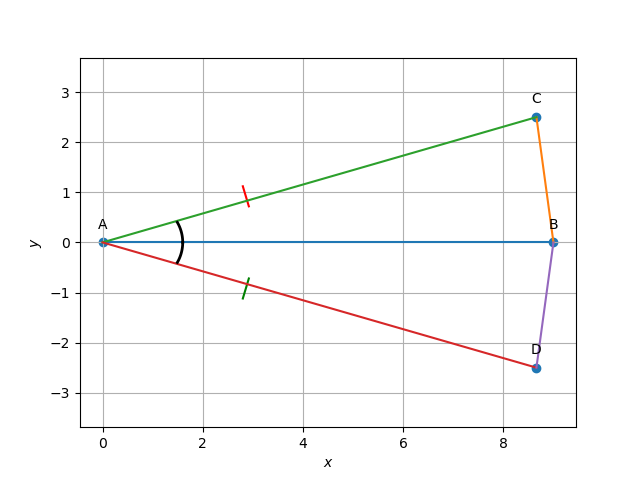
\includegraphics[width=\columnwidth]{figs/graph.png}
	\end{center}
	\caption{}
	\label{fig:Fig}
\end{figure}
\end{document}
